% mnras_template.tex 
%
% LaTeX template for creating an MNRAS paper
%
% v3.0 released 14 May 2015
% (version numbers match those of mnras.cls)
%
% Copyright (C) Royal Astronomical Society 2015
% Authors:
% Keith T. Smith (Royal Astronomical Society)

% Change log
%
% v3.0 May 2015
%    Renamed to match the new package name
%    Version number matches mnras.cls
%    A few minor tweaks to wording
% v1.0 September 2013
%    Beta testing only - never publicly released
%    First version: a simple (ish) template for creating an MNRAS paper

%%%%%%%%%%%%%%%%%%%%%%%%%%%%%%%%%%%%%%%%%%%%%%%%%%
% Basic setup. Most papers should leave these options alone.
\documentclass[fleqn,usenatbib]{mnras}

% MNRAS is set in Times font. If you don't have this installed (most LaTeX
% installations will be fine) or prefer the old Computer Modern fonts, comment
% out the following line
\usepackage{newtxtext,newtxmath}
% Depending on your LaTeX fonts installation, you might get better results with one of these:
%\usepackage{mathptmx}
%\usepackage{txfonts}

% Use vector fonts, so it zooms properly in on-screen viewing software
% Don't change these lines unless you know what you are doing
\usepackage[T1]{fontenc}
\usepackage{ae,aecompl}


%%%%% AUTHORS - PLACE YOUR OWN PACKAGES HERE %%%%%

% Only include extra packages if you really need them. Common packages are:
\usepackage{graphicx}    % Including figure files
\usepackage{amsmath}    % Advanced maths commands
\usepackage{amssymb}    % Extra maths symbols
\usepackage{lscape}
\usepackage{rotating}
\usepackage{esdiff}
\usepackage{esint}
\usepackage{breqn}
%%%%%%%%%%%%%%%%%%%%%%%%%%%%%%%%%%%%%%%%%%%%%%%%%%

%%%%% AUTHORS - PLACE YOUR OWN COMMANDS HERE %%%%%

% Please keep new commands to a minimum, and use \newcommand not \def to avoid
% overwriting existing commands. Example:
%\newcommand{\pcm}{\,cm$^{-2}$}    % per cm-squared

%%%%%%%%%%%%%%%%%%%%%%%%%%%%%%%%%%%%%%%%%%%%%%%%%%

%%%%%%%%%%%%%%%%%%% TITLE PAGE %%%%%%%%%%%%%%%%%%%

% Title of the paper, and the short title which is used in the headers.
% Keep the title short and informative.
\title[Radiative Transfer of Star-Disk Interactions]{Radiative Transfer Simulations of Star-Disk Interactions in T Tauri Systems}

% The list of authors, and the short list which is used in the headers.
% If you need two or more lines of authors, add an extra line using \newauthor
\author[T. J. G. Wilson et al.]{
T. J. G. Wilson,$^{1}$\thanks{E-mail: tjgw201@exeter.ac.uk}
S. Matt,$^{1}$
T. Harries$^{1}$
\\
% List of institutions
$^{1}$College of Engineering, Mathematics and Physical Sciences, Physics Building, Streatham campus,University of Exeter , Exeter EX4 4QL, UK\\
}

% Enter the current year, for the copyright statements etc.
\pubyear{2019}

% Don't change these lines
\begin{document}
\label{firstpage}
\pagerange{\pageref{firstpage}--\pageref{lastpage}}
\maketitle
% Abstract of the paper
\begin{abstract}
\noindent hi there
\end{abstract}

%%%%%%%%%%%%%%%%%%%%%%%%%%%%%%%%%%%%%%%%%%%%%%%%%%

%%%%%%%%%%%%%%%%% BODY OF PAPER %%%%%%%%%%%%%%%%%%

\section{Introduction}
\label{sec:introduction}
Understanding the mechanism by which collapsing interstellar clouds lose angular momentum (hereafter AM), allowing them to form pre-main sequence stars is critical to furthering the study of star and planet formation. Without the loss of AM, the difference in scale of the natal cloud to the protostar would result in a star that was rotating faster than its break up angular velocity~\citep{Hartmann:2016gu}. 


Progenitors to Sun-like objects are T Tauri stars. These are low mass ($\lesssim 2 \textrm{M}_\odot$) pre-main sequence stars which show evidence of accretion from a surrounding accretion disk~\citep{1998ApJ...495..385H}. These young stars ($\lesssim3\times10^{6}~\textrm{yrs}$) have strong H$\alpha$ emission and excess UV and infrared continuum emission~\citep{2005MNRAS.358..671K}. The line profiles exhibit both blue shifted absorption and inverse P Cygni features thought to be evidence of outflows and inflows, respectively. Observed accretion rates ($10^{-9}~\textrm{to}~10^{-7}~{\rm M_{\odot} yr^{-1}}$) are expected to be great enough to transfer enough AM to the star to spin it up to well above break up angular velocity $\Omega_B = \sqrt{GM_{*}/R_{*}^3}$~\citep{2005ApJ...632L.135M} where $M_{\ast}$ and $R_{\ast}$ are the stellar mass and radius respectively. However, a relevant fraction of these stars are rotating well below their rotation limit~\citep{1993A&A...272..176B}, and during the few million years of their accretion phase, their rotation remains fairly constant. In this phase of their evolution, these protostars are still accreting and contracting at rates that should spin them up to break velocity within $\sim10^{6}~{\rm yrs}$~\citep{2009A&A...508.1117Z}. There must be an efficient mechanism to spin down the rotation of the T Tauri stars. 


It is widely accepted that T Tauri stars have accretion disks. Infrared excess and accretion signatures point to their presence. In recent years interferometric observations have confirmed the presence of disks around young stellar objects, for example, the slightly larger Herbig star system shown by \cite{2012ApJ...752...11K} to have a circumstellar disk. The accretion mechanism of T Tauri stars is thought to be dominated by the strong magnetic fields present, $\sim 10^{3}~\textrm{G}$~\citep{2012MNRAS.426.2901K}. \citet{1991ApJ...370L..39K} proposed that the accretion mechanism is similar to that of neutrons stars proposed by~\citet{1977ApJ...217..578G}. The magnetic field truncates the accretion radius at some radii $R_T$ (see Figure~\ref{fig:accretionflow}). where the magnetic and material stresses are of the same order; $B^2/8\pi = p + \rho v^2$, where $B$, $p$, $\rho$ and $v$ are the magnetic field, pressure, density, and velocity respectively~\citep{Romanova:2002hc}. Material is lifted from the disk and free-falls to the stellar surface where it forms a shock region, as the infalling matter exceeds the sound speed of the plasma. The large energy release in these shock zones could be responsible for the high UV excess observed~\citep{2009A&A...508.1117Z}. The accreting matter carries AM to the star and acts to `spin-up' the star. For a given accretion rate $\dot{M}_{acc}$ the `spin-up' rate can be quantified as a torque~\citep{2005ApJ...632L.135M}

\begin{equation}
    \tau_{acc} = \dot{M}_{acc}\sqrt{GM_{\ast}R_{T}}.
    \label{eq:accretion_torque}
\end{equation}
How these T Tauri stars are being braked is still debated~\citep{Hartmann:2016gu} but the possible mechanisms can be split broadly into two types; star-disk interactions and outflows. 


The star-disk interactions rely on Magnetohydrodynamic (MHD) mechanism to remove angular momentum from the star. Magnetic fields threading through the disk and star will provide a negative (or `spin-down') torque if they pass through the accretion disk at radii beyond the corotation radius. The poloidal field lines become twisting as the conductive disk opposes their toroidal passage~\citep{Uzdensky:2002dg} resulting in a `spin-down' torque on the star.  However it not clear whether a `spin-down' torque great enough to match the AM transferred by accretion can be achieved by this magnetic breaking.~\citet{2009A&A...508.1117Z} concluded that for their numerical example the spin down torque from the magnetospheric star-disk ``locking'' could only account for $10\%$ of the spin-up torque from accretion.

\begin{figure}
    \centering
    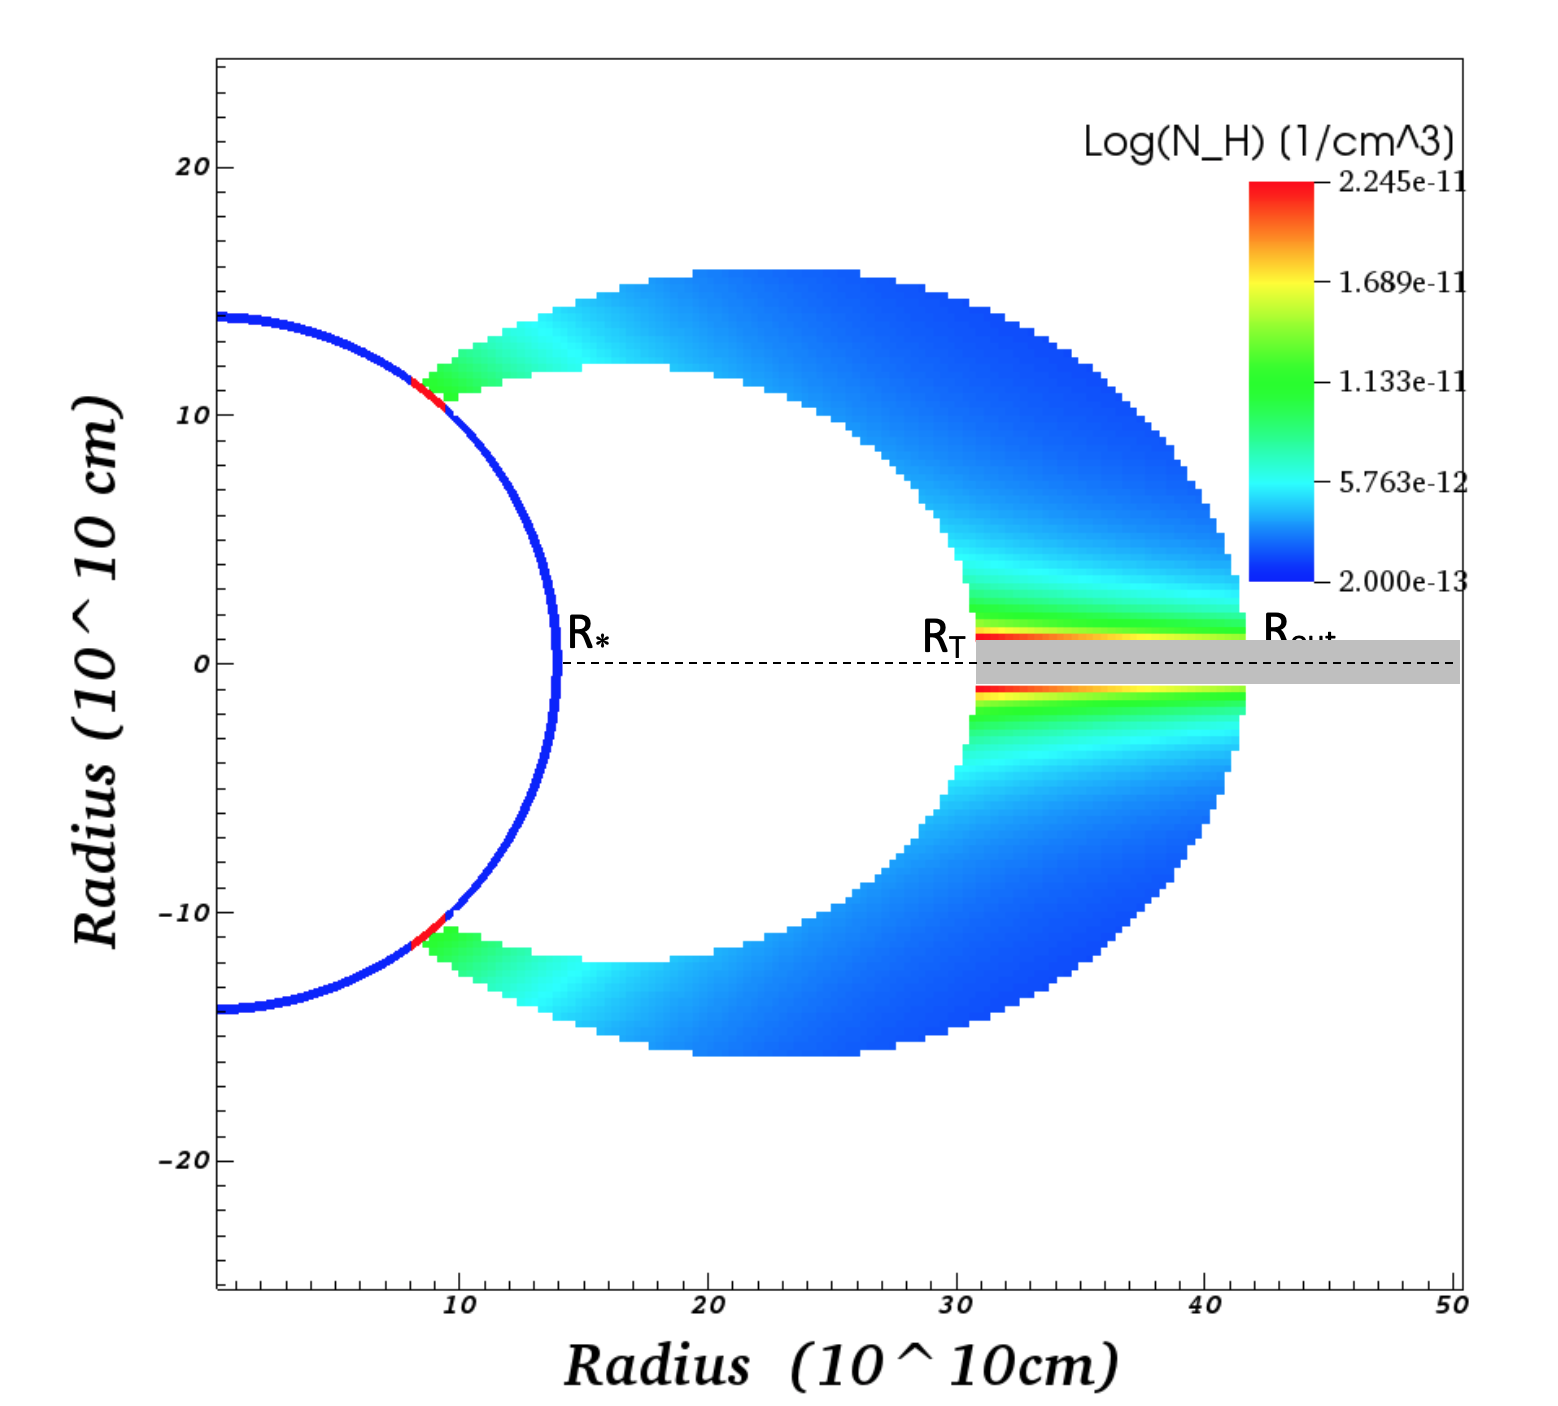
\includegraphics[width=\linewidth]{figures/Accretion}
    \caption{A diagram showing the accretion flow and the density of the flow for a typical set up with an accretion rate of $10^{-7}$ solar masses per year.}
    \label{fig:accretionflow}
\end{figure}

\citep{Shu:tw} proposed that a disk wind along open field lines threading the disk at the corotation radius (``X-wind'') could remove enough AM from the disk that it could render the `spin-up' torque from accretion negligible. This theory still lacks a fully self-consistent dynamical explanation. Another proposed mechanism that the AM can be removed from the star via the interaction of the magnetic field and a stellar wind~\citep[e.g.][]{2005ApJ...632L.135M,Matt:2008bj}. 

\begin{equation}
    \tau_{w} = -\kappa \dot{M}_{w} \Omega_{\ast} r_A^2
    \label{eq:wind_torque}
\end{equation}

Equation~\ref{eq:wind_torque} from~\citep{2005ApJ...632L.135M} gives the torque felt by a star for a given mass loss rate $\dot{M}_{w}$, the stellar rotation rate $\Omega_{\ast}$, the Alfv\'en radius $r_A$ and $\kappa$ a dimensionless quantity accounting for the geometry of the wind. The stellar wind is accelerated by the magnetic field to corotate with the star effectively acting as a solid body out to the Alfv\'en radius from where AM is conserved. This transfers of AM to the wind breaks the star's rotation. The Alfv\'en radius acts like a `lever-arm' slowing the star. Observational evidence of stellar winds have been observed~\citep[e.g.][]{2003ApJ...599L..41E,2006ApJ...646..319E} but the mechanisms driving the winds is still uncertain as T Tauri stars are not active enough to drive stellar winds with a higher enough mass loss rate to match the accretion torque unless a significant proportion ($\sim 36\%$) of the accretion power was used to drive the outflow~\citep{2009A&A...508.1117Z,Matt:2008ic}. The mechanism driving such winds is still uncertain. For example, ~\citet{2008ApJ...689..316C} proposed that turbulent magnetic waves could cause stellar wind with a high enough mass loss rate.


Hence being able to interpret observations for signatures of accretion, winds and most importantly for mass inflow and outflow rates is paramount to constraining our understanding of the physics of early stellar evolution. MHD simulations are extensively used to model the dynamics of T Tauri stars in an attempt to understand physics of the mechanism of AM loss~\citep[e.g.][]{2009A&A...508.1117Z,Matt:2008bj,2019A&A...624A..31C,Romanova:2002hc}. Radiative transfer simulations have been used to model the detectable signatures of the predicted physical models~\citep[e.g.][]{Esau:2014is,2012MNRAS.426.2901K,Kurosawa:2011fh,1998AJ....116..455M,Hartmann:1994tl}. This work intends to concentrate on radiative transfer simulations to complement and supplement the dynamic models of the AWESoMeStars ERC research team.
\begin{figure}
    \centering
    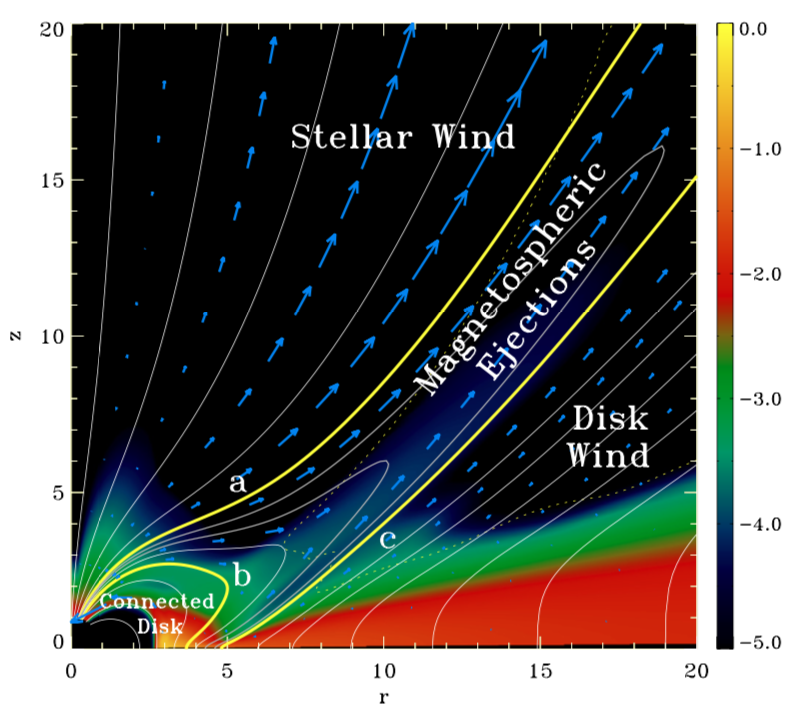
\includegraphics[width=\linewidth]{figures/zanni}
    \caption{MHD simulation snapshot reproduced from~\citet{2009A&A...508.1117Z}, showing the connected disk, stellar and disk winds, and magnetospheric Ejection; another possible mechanism for angular momentum loss. The stellar wind flows along the open magnetic field lines.}
    \label{fig:zanni}
\end{figure}

\section{Radiative Transfer}
\label{sec:radiative}
For all but the most simple of systems modelling the passage of electromagnetic radiation through a medium is a complex problem which has to be solved numerically using radiative transfer simulations~\citep[see][]{2013ARA&A..51...63S}. The propagation of radiation through a medium is effected by the absorption, the emission and the scattering of photons. The equation of radiative transfer is
\begin{equation}
    \diff{I_{\nu}}{\tau_{\nu}} = S_{\nu} - I_{\nu}
\label{eq:RT}
\end{equation}
where $\tau_{\nu}$ is the optical depth of the medium at frequency $\nu$. The specific intensity $I_{\nu}$ is the flux per solid angle per frequency bandwidth. $S_{\nu}$ is the source function which is a ratio of local absorption and emission coefficients.


Past radiative transfer simulations of T Tauri stars have used a Sobolev approximation. The Sobolev approximation assumes that the velocity gradient along a ray is large enough that radiative interactions at any point are determined by the local vicinity. The Sobolev length  or characteristic length $s_0$ of the local vicinity is given by the distance from a point such that the shift in resonant frequency due to the velocity gradient is equal to the half-width of the spectral line profile given by the thermal or turbulent velocity $v_t$
\begin{equation}
    s_0 = v_t \left|\diff{v}{s}\right|{\rm .}
    \label{eq:sobolevlength}
\end{equation}
If the velocity gradient is approximated as $v/R$, where $R$ is the characteristic size of the system and $v$ characteristic large-scale velocity, the Sobolev length can be estimated by $s_0 = R/(v/v_t)$.

The radiative transfer code used here is TORUS~\citep{2019A&C....27...63H}. It has been used~\citep[e.g.][]{2005MNRAS.356.1489S} to model T Tauri systems using the Sobolev approximation. Alternatively, TORUS can use a co-moving frame (CMF) method. Unlike the Sobolev approximation, the CMF code considers the whole system to be potentially affecting the radiative interactions of a given point, not just the local vicinity, so there is no restriction on the velocity field. The full CMF treatment is considerably more computationally expensive than the methods using the Sobolev approximation.

Initial work with TORUS has been modelling the atomic line profiles of a pure hydrogen model of a T Tauri system. The general outline of the computational steps are:
\begin{enumerate}
    \item Initially the grid is populated with gas and radiation sources (see \S\ref{sec:model})
    \item The level populations of the atom in each grid cell are calculated using statistical equilibrium 
    \item The spectral line profiles are then determined from the level populations
\end{enumerate}


\subsection{Statistical Equilibrium}
\label{sec:statistical}

The level populations are calculated assuming statistical equilibrium. The co-moving frame strategy solves for the level populations using a system based on the accelerated Monte Carlo scheme created by~\citet{Hogerheijde:2000wb}. A balance of level populations is achieved in statistical equilibrium. Given by the balance equation
% \begin{multline}
%     \sum_{m<n}\left[ N_m \left( B_{mn}\mathcal{J}_{mn}+N_eC_{mn}\right)-N_n\left( A_{nm}+B_{nm}\mathcal{J}_{mn}+N_eC_{nm}\right) \right]\\+
%     \sum_{m>n}\left[ N_m \left( A_{mn}+B_{mn}J_{mn}+N_eC_{mn}\right)-N_n\left( B_{nm}J_{mn}+N_eC_{nm}\right) \right]\\ +
%     N_{n}^{\ast} \left[ \int_{\nu_{n}}^{\infty} \frac{4\pi}{h\nu}a_{n}(\nu)\left( \frac{2h\nu^3}{c^2}+J_{\nu}\right)\exp{\left(-\frac{h\nu}{k_{B}T}\right)}{\rm d}\nu + N_{e}C_{nk}\right]\\
%     -N{n}\left(\int_{\nu_n}^{\infty} \frac{4\pi}{h\nu}a_{n}(\nu)J_{\nu}{\rm d}\nu +N_{e}C_{nk}\right)=0
% \end{multline}
% where $A_{mn}$ is the Einstein coefficient for spontaneous emission for the quantum levels $m$ and $n$, and $B_{mn}$ and $C_{mn}$ are the Einstein coefficient of stimulated absorption or emission and the collision rate coefficient respectively. $N_n$ is the level population of level $n$ and $N^{\ast}_n$ is the level population given by the Saha-Boltzmann equation for a temperature $T$ and electron density $N_e$. $a_n{\nu}$ is the photoionisation cross section for frequency $\nu$.

\begin{multline}
n_{l}\left[ \sum_{k<l}A_{lk} + \sum_{k\neq l}\left( B_{lk}J_{\nu} +C_{lk}\right)\right] = \\
\sum_{k>l}n_{k}A_{kl} + \sum_{k<\neq l} n_{k}\left(B_{kl}J_{\nu}+C_{kl} \right)
\label{eq:balance}
\end{multline}
where the Einstein coefficients are spontaneous emission $A_{lk}$, stimulated emission and absorption $B_{lk}$, and collision $C_{lk}$ rates for transitions from $l\rightarrow k$. The number density of level $l$ is $n_l$ and $J_{\nu}$ is the mean intensity for frequency $\nu$. The coefficients are not calculated but taken from~\citet{Schoier:2005ja}.

Using a boundary condition of the cosmic microwave background or other bright nearby sources, TORUS solves the balance equation for each grid point iteratively. To determine the level populations a value of the mean intensity is needed, this is calculated by solving the radiative transfer equation along $i$ rays for each grid cell. The mean intensity is given by
\begin{equation}
    J_{\nu}=J_{\nu}^{ext}+J_{\nu}^{int}=\frac{\sum_{i}I_{\nu}^{i}\exp{\left(-\tau_{i}\phi_{\nu}\right)}}{\sum_{i}\phi_{\nu}}+\frac{\sum_{i}S_{\nu}\left(1-\exp{\left(-\tau_{i}\phi_{\nu}\right)}\right)}{\sum_{i}\phi_{\nu}}
    \label{eq:meanintensity}
\end{equation}
a sum of the external intensity $J{\nu}^{ext}$ and an internal intensity $J{\nu}^{int}$. The external mean intensity (from the ambient medium) does not change as the level populations are adjusted whereas the internal intensity changes with the level populations. $\tau_{i}$ is the optical depth along the ray and the source function $S_{\nu}$ is the ration of emission to absorption
\begin{equation}
    S_{\nu}=\frac{n_{k}A_{kl}}{n_{l}B_{lk}-n_{k}B{kl}}.
    \label{eq:sourcefunction}
\end{equation}
The line profile function $\phi_{\nu}$ is characterised by either microtubulant velocity (Gaussian) or by stark broadening (voigt) which is important for optically thick lines such as ${\rm H}\alpha$~\citep{Kurosawa:2011fh}.

Solving for $J_{\nu}$ and hence the level populations is done in two phases. Initially, a set of rays are generated that originate from random positions in the grid cell with random directions and frequencies sampling the line profile function. The radiation field and level populations are iteratively solved till convergence, using the same set of rays; where the root mean square fractional change of the level populations differ by less than $1\%$. By default, TORUS solves for 15 levels with three above that held in local thermal equilibrium. The second phase uses a set of entirely randomly calculated rays, doubling the number of the rays until convergence. The second stage fills in the gaps in the frequency and spatial dimensions of the first stage. 


\subsection{Observed profile calculations}
\label{sec:profilecalculations}
Once the level populations $n_{l}$ are obtained the continuum emissivity $\chi_c$ and opacity $\eta_c$ can easily be determined. The total source function can then be calculated by
\begin{equation}
    S_{\nu} = \frac{\phi_{\nu}S_l+hS_{c}}{\phi_{\nu}+h}
\end{equation}
where the continuum source is $S_{c}=\eta_{c}/\chi_{c}$ and the line source is $S_{l}=\eta_{l}/\chi_{l}$. The line profile $\phi_{\nu}$ as mention above is characterised by either microturbulent velocity broadening or stark broadening. Although when line broadening is negligible this is given by a normal Doppler profile.

TORUS computes a synthetic line profile by placing an image grid (synthetic observer) at a defined location outside of the simulation grid. The grid is used to create a synthetic position-position-velocity atomic line data cube. Rays are calculated with a random position on the image grid intersecting with the simulation framework. Each ray is weighted by the number of rays originating in the same image grid cell.

The specific intensity $I_{\nu}$ for a ray along $t$ is determined from
\begin{equation}
I_{\nu} = I_{0}{\rm e}^{-\tau_{\infty}} + \int^{-\tau_{\infty}}_{0}S_{\nu}\left(\tau_{\nu}'\right){\rm e}^{-\tau_{\nu}'}{\rm d}\tau_{\nu}'
\end{equation}
where $\tau_{\nu}$ is the optical depth and $\tau_{\infty}$ is the total optical depth from the observer to the initial integration point.$I_0$ is the boundary intensity, $I_0=0$ unless the ray intersects with the stellar surface, where $I_0$ is determined from stellar atmosphere model given by~\citet{1979ApJS...40....1K}. If a ray hits the bright accretion ring on the stars surface, the intensity is calculated as a black body for the rings temperature and observed frequency.

The optical depth $\tau_{\nu}$ along a path $t$ is given by
\begin{equation}
    \tau_{\nu} = \int_{t}^{t_{\infty}} \chi_{\nu}\left(t' \right){\rm d}t'
\end{equation}
where $t_{\infty}$ is the total distance to the observer or the outer boundary closest to the observer. The optical depth is integrated across the grid cells of the adaptive mesh set up by TORUS. For optically thick regions the emissivity and opacity are interpolated to additional points within the cell to keep ${\rm d}\tau_{\nu} > 0.05$. 

The observed flux for a cell of the grid image is the summation of the specific intensities for all rays ending in the cell, times their weighting and the area of the cell.

\section{The models}
\label{sec:model}

TORUS uses an adaptive mesh refinement (AMR) to create a grid of cell through which it can compute the level populations and intensities.  A numerical grid representing the physical space of the simulation is created, and the coarseness of the cells is adapted to balance both the accuracy of the simulation and the efficiency. Too coarse a grid will lose details and may miss features such as areas of high opacity, whereas too fine a grid will run excessively slow and consume large amounts of computational resources.

The work here presents the simulation of T Tauri star-disk systems. For this, the mesh is populated with a star, disk, accretion flow and potentially outflows. The density, temperatures and velocities fields are defined to simulate a T Tauri system. Future work will load in this data as an output from MHD simulations, but at present, this is done analytically. TORUS can include He in the simulations although this is as yet unvalidated. 

The star is placed at the origin of the grid and assumed to have an atmosphere as modelled by~\citet{1979ApJS...40....1K}. The disk is treated as a geometrically thin, optically thick disk. Rays that intersect with it are terminated, no continuum or dust emission from the disk is currently included in the model, although this will be implemented in future work.

\subsection{Accretion Funnel}
\label{sec:accretion}
The geometry and parameters of the accretion flow are similar to those described by \citet{1998ApJ...495..385H}. The inner radius of the accretion flow is where the disk is truncated $R_{T}$. The outer radius $R_{\rm out}$ of the accretion flow is assumed to be the corotation radius, to avoid a ring of rapid acceleration where the disk spins up or down to match the magnetic field which is rotating as a rigid body with the star. Although MHD simulations show twisting of the magnetic fields~\citep[e.g.][]{Uzdensky:2002dg} this is ignored in, and the magnetic field is assumed to have only a poloidal component.

The accreting matter free flows following the dipole magnetic field impacting on the surface of the star creating a hot spot. The temperature of the hot spot is calculated from the potential energy liberated as the matter falls to a lower radius.

The geometry of the field is as explored by~\citet{1991ApJ...370L..39K,1977ApJ...217..578G}. For a starting radius at the equator, $R_{0}$ in spherical coordinates, with a colatitude $theta$ the dipole streamline is given by
\begin{equation}
    R = R_{0}\sin^{2}(\theta).
\end{equation}
The poloidal magnetic field component at radius $R$ is
\begin{equation}
    B_{p}(R,\theta) = \mu R^{-3}\sqrt{4-3\sin^{2}(\theta )}
\end{equation}
where $\mu$ is the magnetic dipole moment. Finding the unit vector of the $B_p$ and converting to Cartesian coordinates gives the components of the accretion flows unit vector
\begin{equation}
     \mathbf{\hat{v}_p} = \frac{1}{\sqrt{4-3\sin^2\theta}}\left(3\sin(\theta)\sqrt{1-\sin^2\theta}\mathbf{\hat{x}}+(2-3\sin^2\theta)\mathbf{\hat{z}}\right).
\end{equation}
The magnitude of the flow at $R$ is calculated from the change in potential energy,
\begin{equation}
    v_p = \sqrt{2GM_{\ast}(\frac{1}{R} - \frac{1}{R_0})}
\end{equation}
the velocity of the flow is $\mathbf{v_p}=v_p\mathbf{\hat{v}_p}$.
The density of the accretion flow is taken from~\citep{Hartmann:1994tl}. For an accretion rate $\dot{M}_{\rm acc}$ the density at radius $R$ is given to be
\begin{equation}
    \rho = \frac{\dot{M}_{\rm acc}}{4\pi(1/R_T - 1/R_{\rm out})}\frac{R^{-5/2}}{\sqrt{2GM_{\ast}}}\frac{\sqrt{4-3\sin^2\theta}}{\sqrt{1-\sin^2\theta}}
\end{equation}
The temperature distribution of the accretion flow is more problematic. The synthetic emission lines are very sensitive to temperature variations in these regions but exact mechanism of heating is debated. The temperature profile adopted is similar that used by~\citet{Hartmann:1994tl,1998ApJ...492..743M} which assumes a volumetric heating $\propto R^{-3}$ balanced by radiative cooling. Figure~\ref{fig:density} shows the temperature, density and velocity distributions used in our models compared to those used by~\citet{1998ApJ...492..743M}.
\begin{figure}
    \centering
    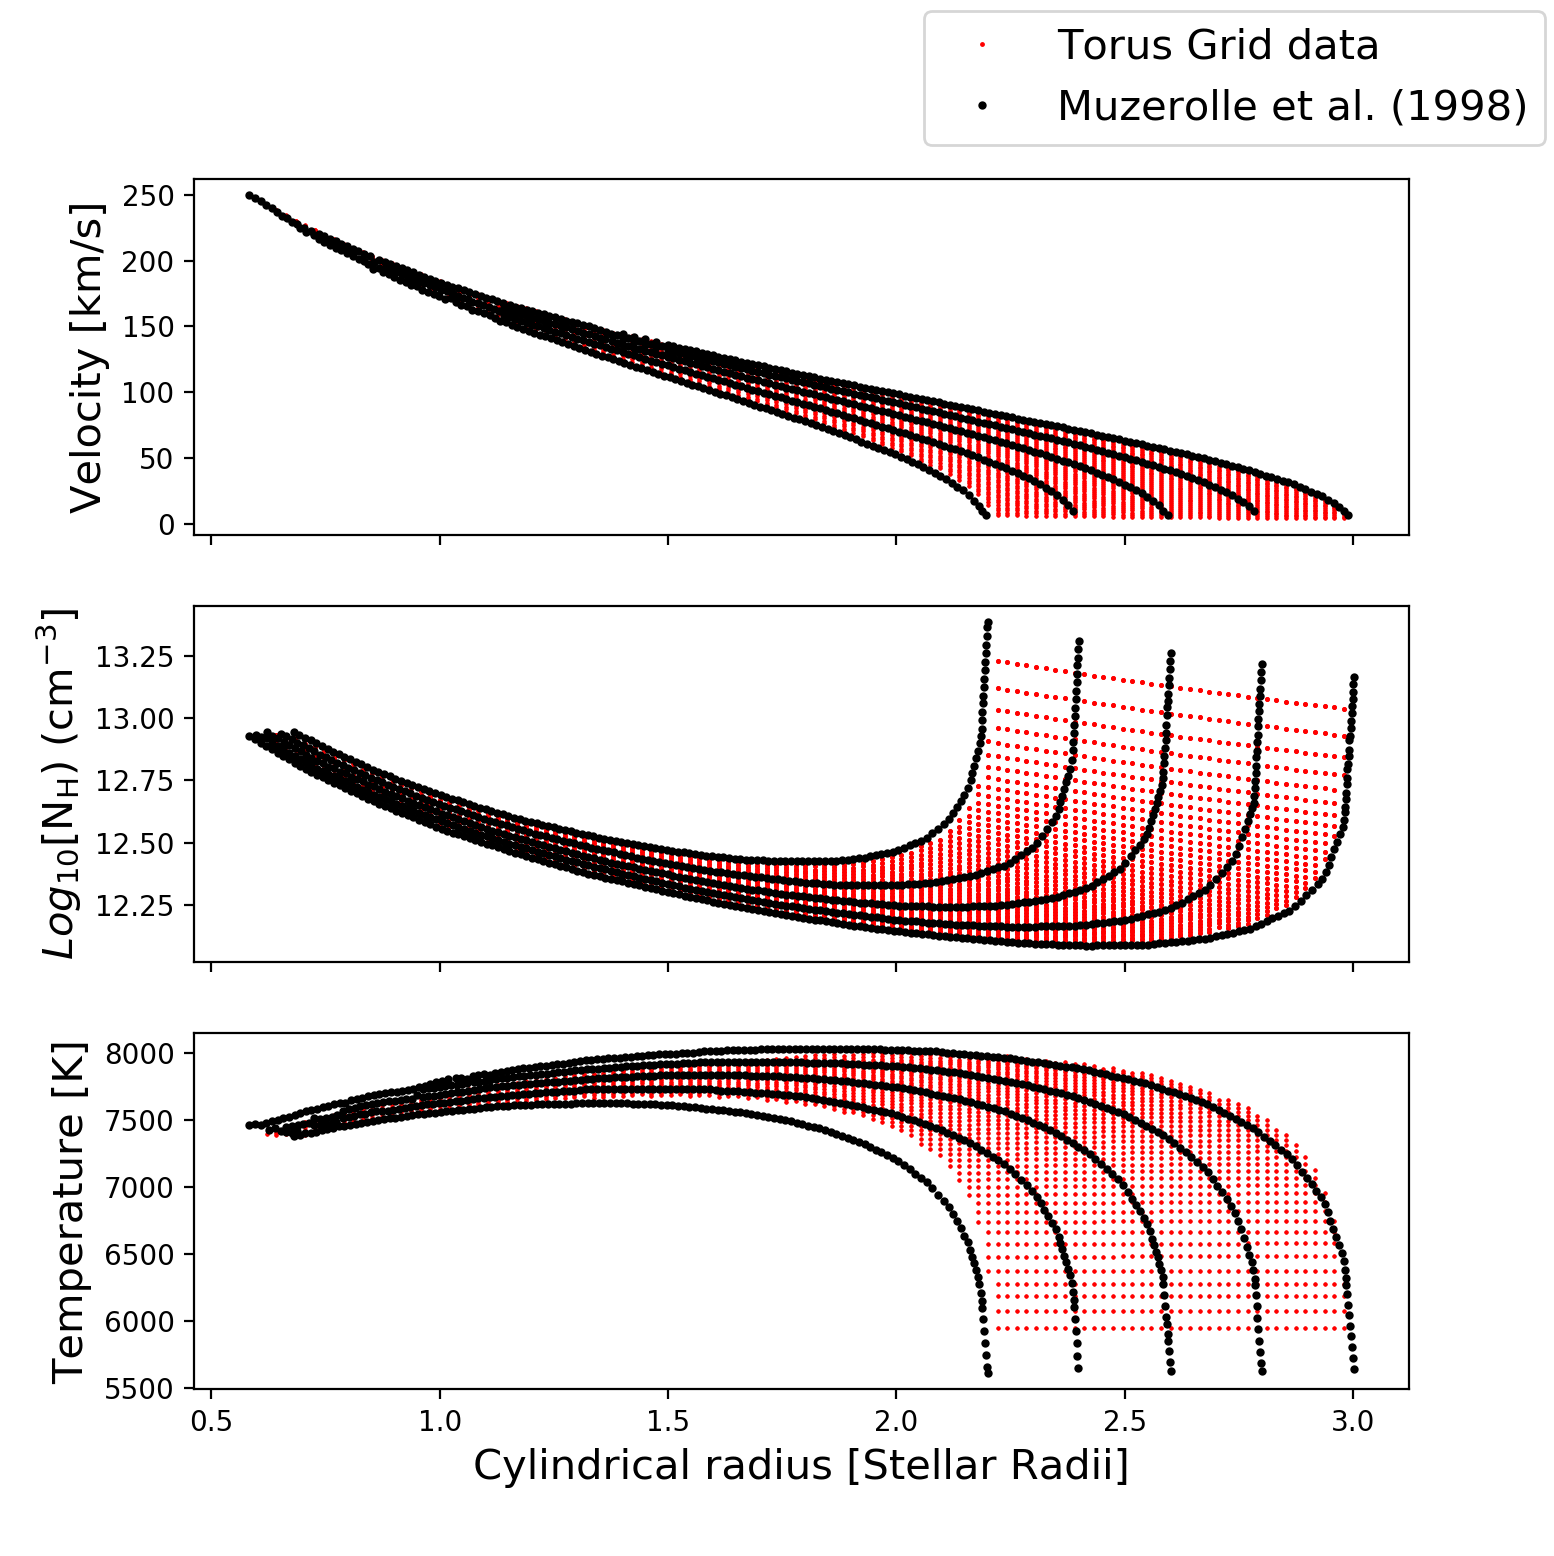
\includegraphics[width=\linewidth,trim={0 1cm 0 0},clip]{figures/density}
    \caption{A plot of the velocity (top), density (middle) and temperature (bottom) distribution in the accretion flow plotted against the radius. Red marks are taken from the TORUS grid points and the black points are the distribution used by~\citet{1998ApJ...492..743M}}
    \label{fig:density}
\end{figure}

Based on the work by~\citet{Mahdavi:1998fw} TORUS allows 3D models to have an offset $\beta$ to the magnetic dipole from the rotation axis. The result of this is a preferable accretion on opposite sides of the star, see Figure~\ref{fig:3Doffset}.
\begin{figure}
    \centering
    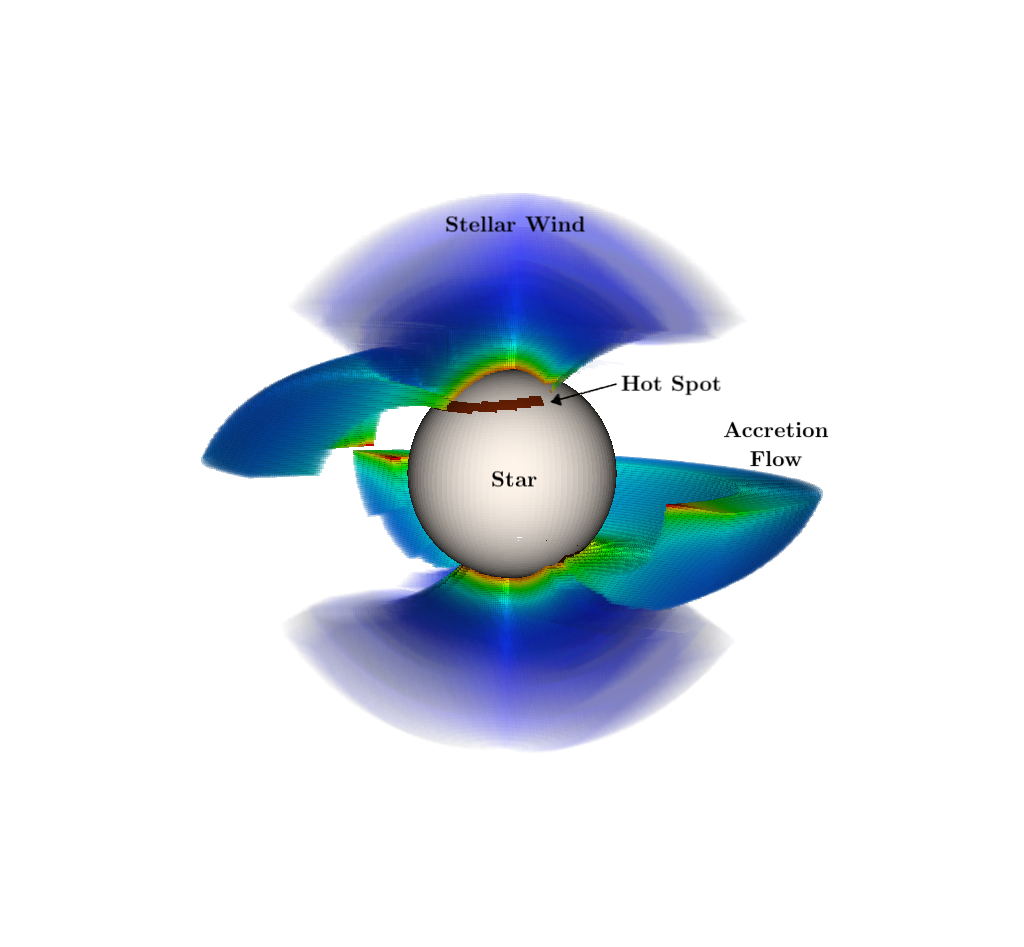
\includegraphics[width=\linewidth,trim={2cm 1cm 2cm 1cm},clip]{figures/3Doffset}
    \caption{A 3D rendering of T Tauri star set up where a 10 degree magnetic offset has been stipulated. The accretion flow is in opposite hemispheres, favouring the shortest route to stellar surface. Part of the wind and accretion flow have been cut away showing the star and hot spot zones.}
    \label{fig:3Doffset}
\end{figure}

\subsection{Stellar Wind}
\label{sec:wind}
TORUS contained the code to initialise spherical isotropic stellar wind into the simulation grid. However, this is an unphysical description of possible stellar winds when in conjunction with disks and magnetospheric accretion. A better approximation is a wind that flows along the open magnetic field lines above the magnetospheric accretion funnel flow~\citep[e.g.][]{2009A&A...508.1117Z,2012MNRAS.426.2901K} see Figure~\ref{fig:zanni}.

A newly updated wind system is now available in TORUS, which allows the system to have a non-spherically symmetric polar wind. Similar work by \citet{Kurosawa:2011fh} implemented a polar stellar wind starting from a radius $R_0$ above the stellar surface the reason for the wind not originating at the stellar surface was that it restricted the wind to a half opening angle of $\sim 35^{\circ}$. The stellar wind presented here overcomes this problem by allowing the wind to follow the dipole magnetic field lines out till they reach the desired half opening angle, at which point the wind becomes radial~\ref{fig:wind}.
\begin{figure}
    \centering
    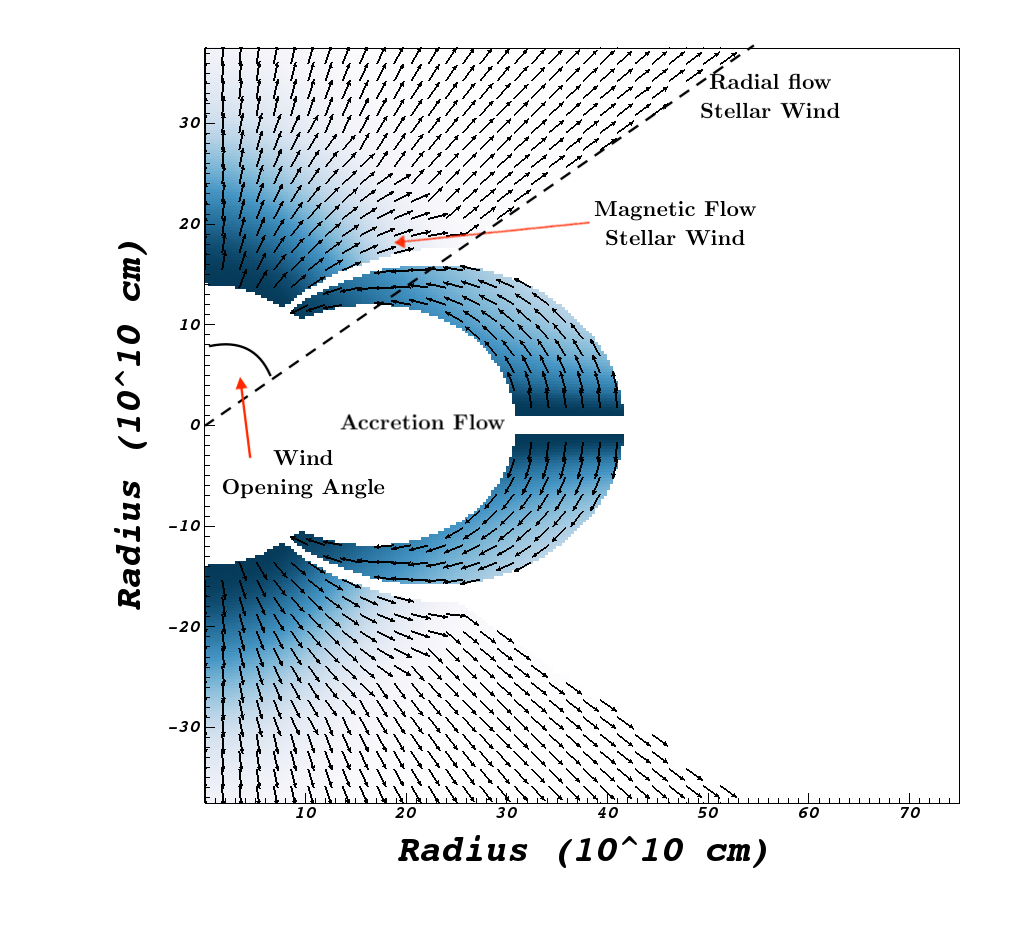
\includegraphics[width=\linewidth]{figures/wind}
    \caption{Depiction of the stellar wind used by TORUS. The wind follows the poloidal direction of the dipole magnetic field until it reaches the half-width opening angle required.}
    \label{fig:wind}
\end{figure}
The magnitude of the poloidal component of the stellar wind velocity is given a beta law,
\begin{equation}
    V_{p}(R) = V_{\rm min} + \left( V_{\rm max}-V_{\rm min}\right)\left(1-\frac{R_{\ast}}{R}\right)^{\beta}
    \label{eq:beta}
\end{equation}
where $V_{\rm min}$ and $V_{\rm max}$ are the starting and end velocities of the wind. $\beta$ is a parameter that can be tuned to find the correct wind gradient. The toroidal velocity component $V_{T}(R)$ is derived from the rotation rate of the star. The wind is threaded by a magnetic field and the stellar wind is assumed to corotate as a rigid body with the star out till the Alfv\'en radius. Beyond this the wind conserves angular momentum, the velocity decreasing as a function of $\propto 1/R$, see Figure~\ref{fig:polVel}.
\begin{figure}
    \centering
    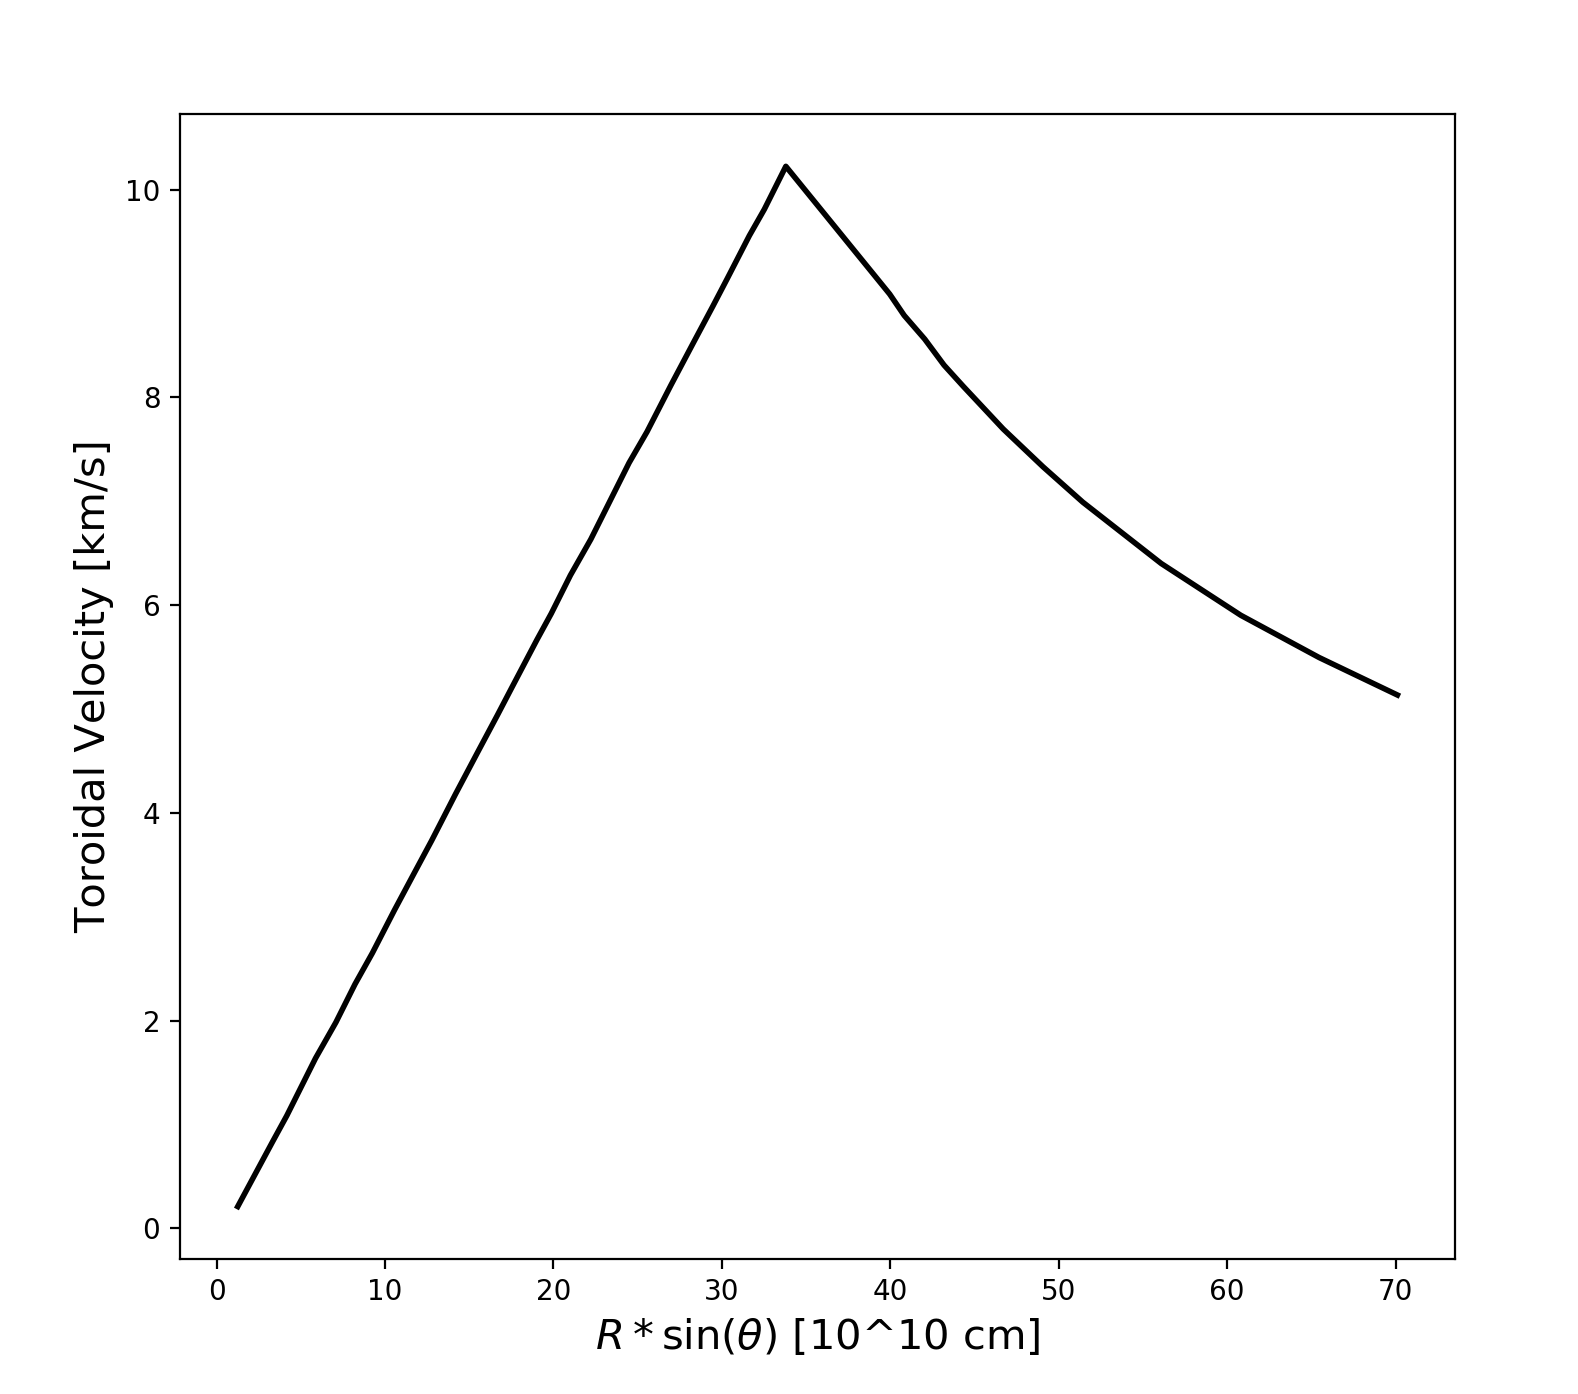
\includegraphics[width=\linewidth]{figures/torVel}
    \caption{An example of the toroidal velocity magnitude profile for a stellar wind. The point where the wind stops acting as rigid body with the star is an approximation of the Alfv\'en radius.}
    \label{fig:polVel}
\end{figure}

The density of the stellar wind is derived from the input mass loss rate $\dot{M}_{\rm wind}$. The wind density goes with $\rho \propto \dot{M}_{\rm wind}/VA$ where is $V$ is the velocity of the wind normal to the surface $A$. Up to the Alfv\'en radius the wind can be assumed to be contained within a diverging flux tube, the magnetic flux of a dipole diverges at a rate of $1/R^3$ hence the surface $A \propto R^3$ and the density decreases as $\propto 1/R^3$. Beyond the Alfv\'en radius, the surface $A$ increases as a spherical cap (radial flow) so the density decreases $\propto 1/R^2$. The density is computed by
\begin{equation}
    \rho = \frac{1}{2}\frac{\dot{M}_{\rm wind}}{V(R)A_{\ast}}\left( \frac{R_{\ast}}{R}\right)^3
\end{equation}
for radii $R_{\ast}\leq R < R_{\rm A}$ where $A_{\ast}$ is the surface area at one pole of the star from which the stellar wind is launched. For radii greater than the Alfv\'en radius $R_{\rm A}$ the density is given by

\begin{equation}
    \rho = \frac{1}{2}\frac{\dot{M}_{\rm wind}}{V(R)A_{A}}\left( \frac{R_{A}}{R}\right)^2
\end{equation}
where $A_A$ is the spherical cap surface area with radius $R_A$ such that $A_A = 2\pi R^2 (1-\cos\theta_{\rm open})$ where $\theta_{\rm open}$ is the user defined max opening angle of the wind (see Figure~\ref{fig:wind}). Should the magnetic dipole be offset from the rotation axis the wind follows the tilted magnetic field before becoming radial.

\section{Current Results}
\label{sec:results}

The current work has been implementing the stellar wind (See~\ref{sec:wind}) code and replicating the results of~\citet{1998ApJ...492..743M}. Their results for a cylindrically symmetric T Tauri star with an accretion flow but no stellar wind or disk winds were computed using the Sobolev approximation and are in agreement with~\citet{Hartmann:1994tl}.

Figure~\ref{fig:muzerolle} shows the figure that we are trying to replicate with TORUS using the CMF module (see \S\ref{sec:statistical}) of the radiative transfer code. 
\begin{figure}
    \centering
    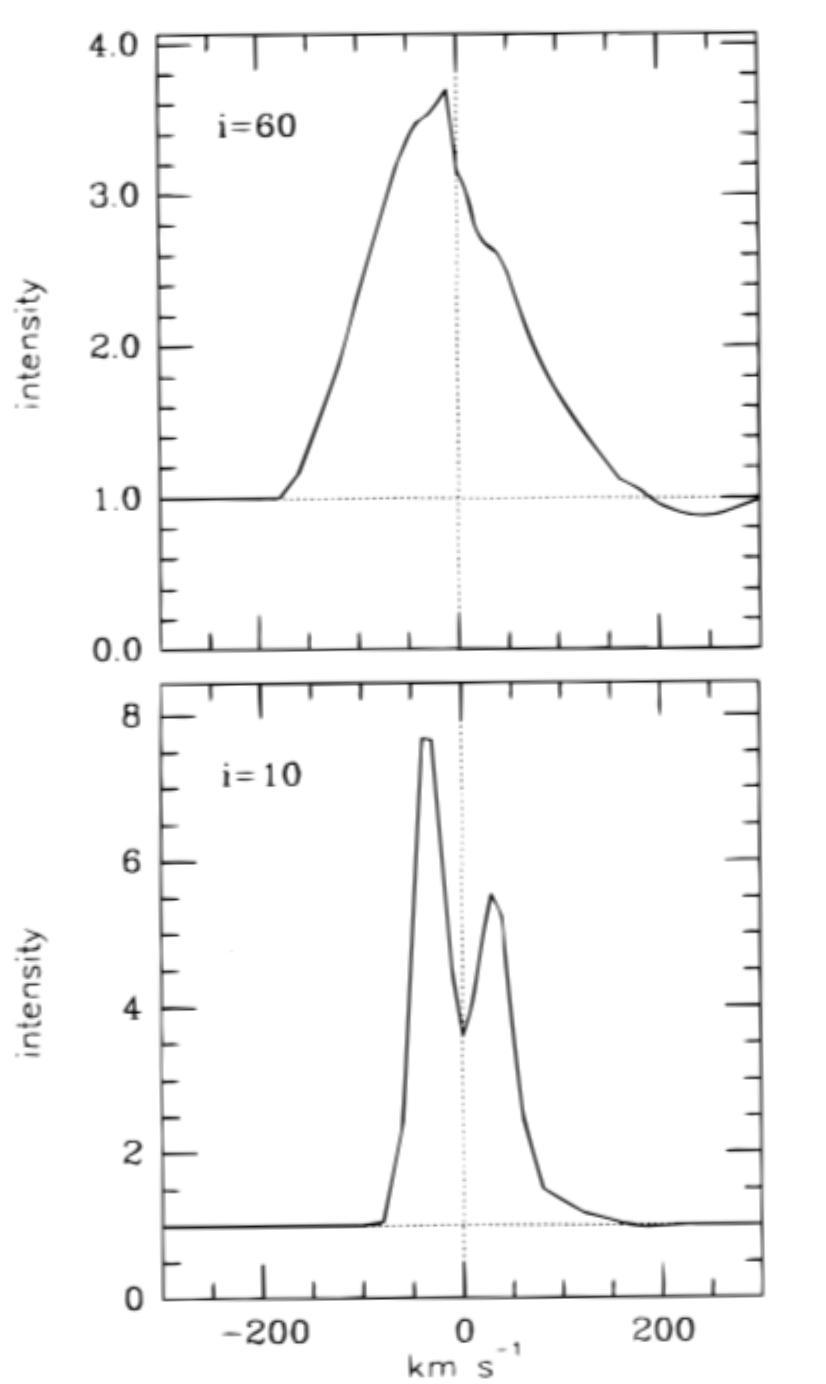
\includegraphics[width=\linewidth]{figures/muz}
    \caption{${\rm H}\alpha$ line profile from \citet{1998ApJ...492..743M} for inclinations of $10^{\circ}$  (bottom) and $60^{\circ}$ (top). These show the red shifted absorption features expected from a accretion flow.}
    \label{fig:muzerolle}
\end{figure}

The model used to create the ${\rm H}\alpha$ line profiles shown in Figure~\ref{fig:muzerolle} has the following characteristics. The mass accretion rate is $10^{-7} ~{\rm \dot{M}_{\odot}yr^{-1}}$ with a maximum accretion flow temperature of $7500~\textrm{K}$. The star's features were $R_{\ast}=2~{\rm R_{\odot}}$, $M_{\ast}=0.8~{\rm M_{\odot}}$, the photosphere temperature was $4000~\textrm{K}$ and the maximum hot spot temperature $7200~\textrm{K}$, the stellar atmosphere was modelled as a blackbody. The magnetosphere had an inner radius of $2.2~{\rm R_{\ast}}$ and an outer radius of $3~{\rm R_{\ast}}$. Stellar rotation is neglected and assumed to be negligible.

The T Tauri star model set up for our simulation run with TORUS use the same physical properties apart from, the stellar photosphere is modelled as given by~\citet{1979ApJS...40....1K} rather than a blackbody. The temperature distribution within the accretion flow differs at the outer radii from that used by~\citet{1998ApJ...492..743M} see Figure~\ref{fig:density}.

Initial tests of the model were hampered by several bugs within the CMF code and what broadening parameters should be used. The current best ${\rm H}\alpha$ line profile using microtubulant broadening with a characteristic velocity of $2~{\rm kms^{-1}}$ is shown in Figure~\ref{fig:bestline}

\begin{figure*}
    \centering
    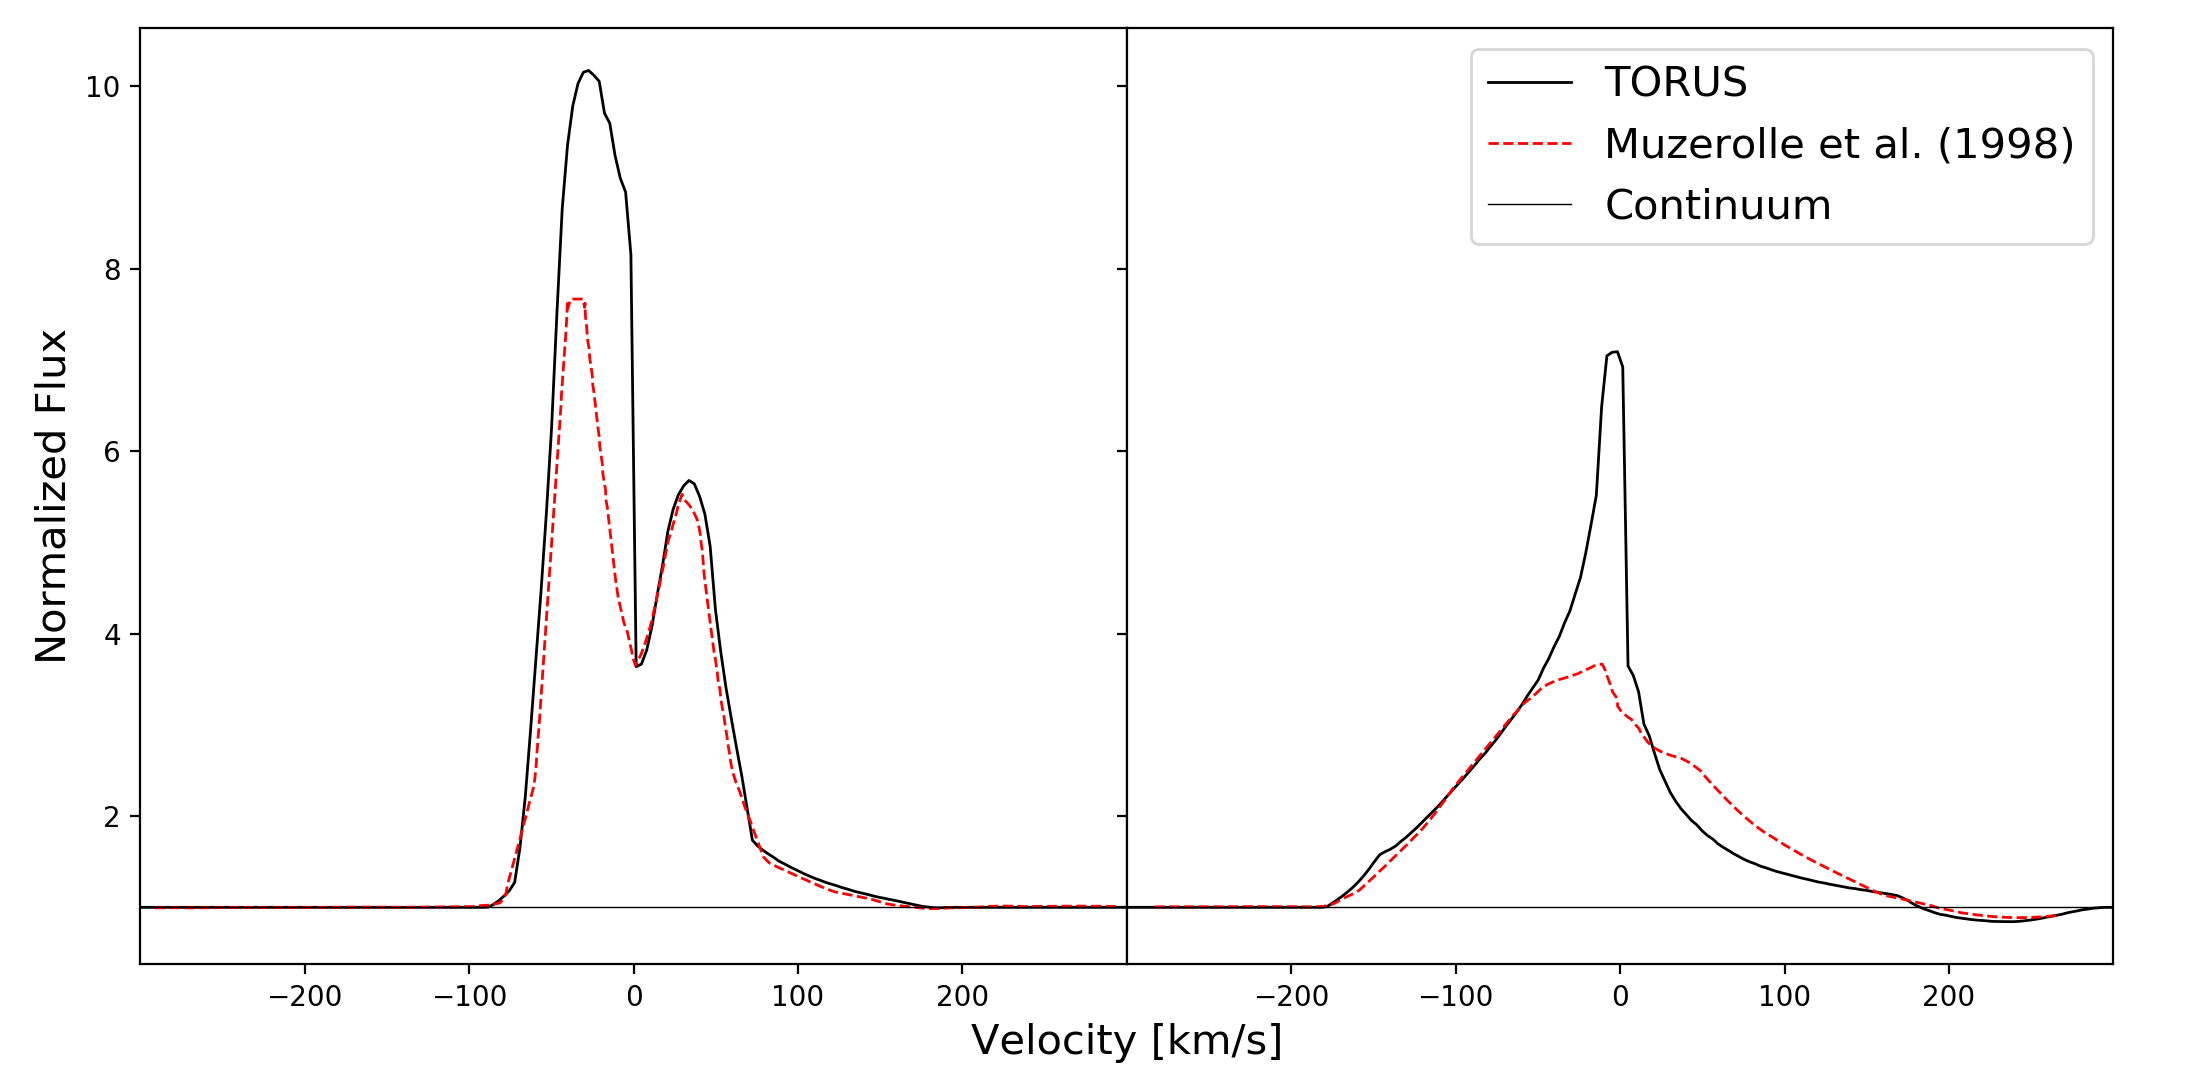
\includegraphics[width=\linewidth]{figures/results}
    \caption{${\rm H}\alpha$ line profiles from TORUS (black line) and~\citep{1998ApJ...492..743M} (red dashed) with viewing angles of $10^{\circ}$ (left panel) and of $60^{\circ}$ (right panel). The}
    \label{fig:bestline}
\end{figure*}

Our results display a the characteristic Inverse P-Cygni profile especially when viewed from an inclination of $60^{\circ}$. However, our results show a much stronger emission from that of\citep{1998ApJ...492..743M} for emissions with a low Doppler shift. The line widths are similar and for an inclination of $10^{\circ}$ our results show the expected double peak.

\section{Conclusions}
\label{sec:conclusions}
The propriety work to using radiative transfer simulations to model the observational signatures T Tauri stars by creating synthetic atomic line profiles has been undertaken. These results will potentially lead to new insights into the mechanism of angular momentum loss in these stars and further our understanding of the evolution of pre-main sequence stars.

Work to replicate the results of~\citep{1998ApJ...492..743M} has yielded line profiles with similar signatures but further investigation is needed to determine whether the differences are due to errors in the TORUS code or are the result of the different radiative transfer system used.
The code to implement a polar stellar wind in the set up of the T Tauri star model has been written and integrated with the existing TORUS code. It is still unvalidated but future work could compare the results to those of~\citet{Kurosawa:2011fh}.
%\section*{Acknowledgements}


%%%%%%%%%%%%%%%%%%%%%%%%%%%%%%%%%%%%%%%%%%%%%%%%%%

%%%%%%%%%%%%%%%%%%%% REFERENCES %%%%%%%%%%%%%%%%%%

% The best way to enter references is to use BibTeX:
\clearpage
\bibliographystyle{mnras}
\bibliography{library} % if your bibtex file is called example.bib

%%%%%%%%%%%%%%%%%%%%%%%%%%%%%%%%%%%%%%%%%%%%%%%%%%

%%%%%%%%%%%%%%%%% APPENDICES %%%%%%%%%%%%%%%%%%%%%

%\appendix
%\section{Some extra material}


%%%%%%%%%%%%%%%%%%%%%%%%%%%%%%%%%%%%%%%%%%%%%%%%%%

% Don't change these lines
\bsp    % typesetting comment
\label{lastpage}
\end{document}

% End of mnras_template.tex